% Options for packages loaded elsewhere
\PassOptionsToPackage{unicode}{hyperref}
\PassOptionsToPackage{hyphens}{url}
\PassOptionsToPackage{dvipsnames,svgnames,x11names}{xcolor}
%
\documentclass[
  letterpaper,
  DIV=11,
  numbers=noendperiod]{scrartcl}

\usepackage{amsmath,amssymb}
\usepackage{iftex}
\ifPDFTeX
  \usepackage[T1]{fontenc}
  \usepackage[utf8]{inputenc}
  \usepackage{textcomp} % provide euro and other symbols
\else % if luatex or xetex
  \usepackage{unicode-math}
  \defaultfontfeatures{Scale=MatchLowercase}
  \defaultfontfeatures[\rmfamily]{Ligatures=TeX,Scale=1}
\fi
\usepackage{lmodern}
\ifPDFTeX\else  
    % xetex/luatex font selection
\fi
% Use upquote if available, for straight quotes in verbatim environments
\IfFileExists{upquote.sty}{\usepackage{upquote}}{}
\IfFileExists{microtype.sty}{% use microtype if available
  \usepackage[]{microtype}
  \UseMicrotypeSet[protrusion]{basicmath} % disable protrusion for tt fonts
}{}
\makeatletter
\@ifundefined{KOMAClassName}{% if non-KOMA class
  \IfFileExists{parskip.sty}{%
    \usepackage{parskip}
  }{% else
    \setlength{\parindent}{0pt}
    \setlength{\parskip}{6pt plus 2pt minus 1pt}}
}{% if KOMA class
  \KOMAoptions{parskip=half}}
\makeatother
\usepackage{xcolor}
\setlength{\emergencystretch}{3em} % prevent overfull lines
\setcounter{secnumdepth}{-\maxdimen} % remove section numbering
% Make \paragraph and \subparagraph free-standing
\ifx\paragraph\undefined\else
  \let\oldparagraph\paragraph
  \renewcommand{\paragraph}[1]{\oldparagraph{#1}\mbox{}}
\fi
\ifx\subparagraph\undefined\else
  \let\oldsubparagraph\subparagraph
  \renewcommand{\subparagraph}[1]{\oldsubparagraph{#1}\mbox{}}
\fi


\providecommand{\tightlist}{%
  \setlength{\itemsep}{0pt}\setlength{\parskip}{0pt}}\usepackage{longtable,booktabs,array}
\usepackage{calc} % for calculating minipage widths
% Correct order of tables after \paragraph or \subparagraph
\usepackage{etoolbox}
\makeatletter
\patchcmd\longtable{\par}{\if@noskipsec\mbox{}\fi\par}{}{}
\makeatother
% Allow footnotes in longtable head/foot
\IfFileExists{footnotehyper.sty}{\usepackage{footnotehyper}}{\usepackage{footnote}}
\makesavenoteenv{longtable}
\usepackage{graphicx}
\makeatletter
\def\maxwidth{\ifdim\Gin@nat@width>\linewidth\linewidth\else\Gin@nat@width\fi}
\def\maxheight{\ifdim\Gin@nat@height>\textheight\textheight\else\Gin@nat@height\fi}
\makeatother
% Scale images if necessary, so that they will not overflow the page
% margins by default, and it is still possible to overwrite the defaults
% using explicit options in \includegraphics[width, height, ...]{}
\setkeys{Gin}{width=\maxwidth,height=\maxheight,keepaspectratio}
% Set default figure placement to htbp
\makeatletter
\def\fps@figure{htbp}
\makeatother

\usepackage{fancyhdr}
\KOMAoption{captions}{tableheading}
\makeatletter
\@ifpackageloaded{caption}{}{\usepackage{caption}}
\AtBeginDocument{%
\ifdefined\contentsname
  \renewcommand*\contentsname{Table of contents}
\else
  \newcommand\contentsname{Table of contents}
\fi
\ifdefined\listfigurename
  \renewcommand*\listfigurename{List of Figures}
\else
  \newcommand\listfigurename{List of Figures}
\fi
\ifdefined\listtablename
  \renewcommand*\listtablename{List of Tables}
\else
  \newcommand\listtablename{List of Tables}
\fi
\ifdefined\figurename
  \renewcommand*\figurename{Figure}
\else
  \newcommand\figurename{Figure}
\fi
\ifdefined\tablename
  \renewcommand*\tablename{Table}
\else
  \newcommand\tablename{Table}
\fi
}
\@ifpackageloaded{float}{}{\usepackage{float}}
\floatstyle{ruled}
\@ifundefined{c@chapter}{\newfloat{codelisting}{h}{lop}}{\newfloat{codelisting}{h}{lop}[chapter]}
\floatname{codelisting}{Listing}
\newcommand*\listoflistings{\listof{codelisting}{List of Listings}}
\makeatother
\makeatletter
\makeatother
\makeatletter
\@ifpackageloaded{caption}{}{\usepackage{caption}}
\@ifpackageloaded{subcaption}{}{\usepackage{subcaption}}
\makeatother
\ifLuaTeX
  \usepackage{selnolig}  % disable illegal ligatures
\fi
\usepackage{bookmark}

\IfFileExists{xurl.sty}{\usepackage{xurl}}{} % add URL line breaks if available
\urlstyle{same} % disable monospaced font for URLs
\hypersetup{
  pdftitle={Midterm 1},
  pdfauthor={STAT425, Fall 2023},
  colorlinks=true,
  linkcolor={blue},
  filecolor={Maroon},
  citecolor={Blue},
  urlcolor={Blue},
  pdfcreator={LaTeX via pandoc}}

\title{Midterm 1}
\author{STAT425, Fall 2023}
\date{2023-10-19}

\begin{document}
\maketitle

\pagestyle{fancy} \fancyhead[LH]{Midterm 1} \fancyhead[RH]{STAT425, Fall 2023}

\textbf{Instructions}: read each problem carefully and provide answers
in the space below. Your answers should display your reasoning clearly.
If you use results from class in your answer, you can simply write, ``by
a theorem from class\ldots{}'', and need not identify the result by
name. You do not need to justify small steps in this way. You also do
not need to calculate decimals or perform any burdensome calculations,
but you should simplify your answers as much as possible. Please feel
free to ask any clarifying questions about the problems. You have 50
minutes to complete the exam. Good luck!

\begin{enumerate}
\def\labelenumi{\arabic{enumi}.}
\tightlist
\item
  Consider a dart board comprising concentric circles with radii
  \(r, \frac{2}{3}r, \frac{1}{3}r\), as depicted below. Suppose this
  board is mounted on a unit square, and that for an inexperienced
  player, the probability of hitting each region is simply the area of
  that region. Assume that a throw will land within the unit square. The
  scoring rules are: 0 points are awarded if the board is missed, 1
  point is awarded for hitting the outermost circle, 2 points are
  awarded for hitting the middle circle, and 3 points are awarded for
  hitting the inner circle. Find an expression for the probability of
  scoring \(i\) points on a single throw and show (or argue) that it is
  a valid probability measure.
\end{enumerate}

\begin{center}
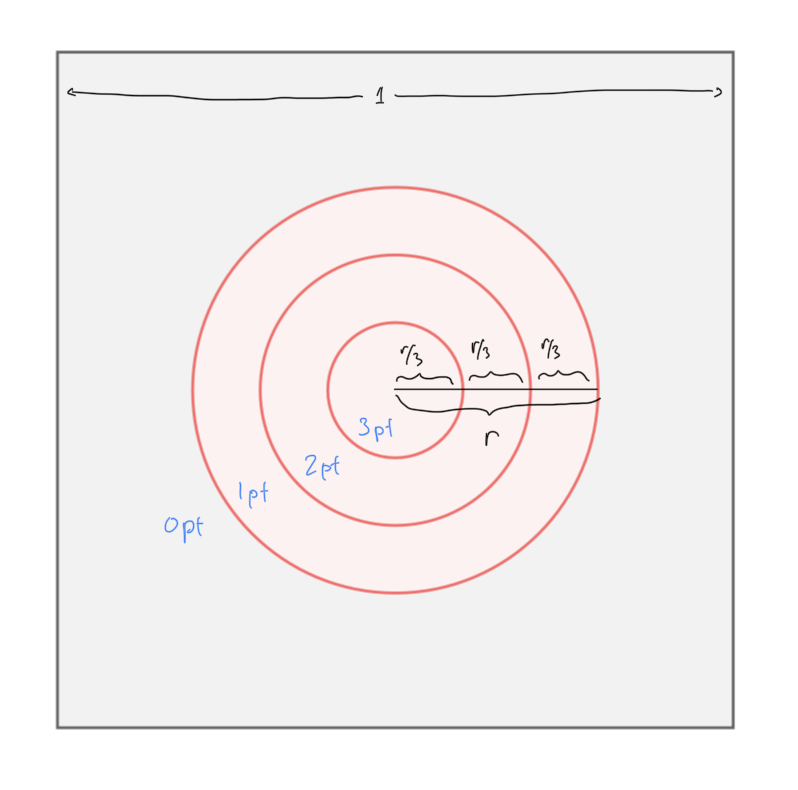
\includegraphics[width=3.125in,height=\textheight]{Dartboard.png}
\end{center}

\begin{enumerate}
\def\labelenumi{\arabic{enumi}.}
\setcounter{enumi}{1}
\item
  Imagine you work a summer job at a theme park. At the entrance there
  are 5 ticket booths, and on a particular morning, there are 200 people
  waiting at the entrance. Everyone waiting must choose one line and buy
  a ticket individually. You're working at the first ticket booth, and
  it takes you exactly 2 minutes to process each transaction. After you
  finish selling the morning tickets, you'll take a break. If customers
  select their lines at random and no new customers arrive, what is the
  probability that you'll be on break in exactly an hour?
\item
  Suppose you've developed a machine learning model to classify activity
  patterns as ``at work'' or ``not at work'' based on user cell phone
  data. In testing prior to deployment, you assess performance on
  timepoints sampled from 1000 users whose information was not used in
  the development of the model; of those, 800 users were working during
  the sampled timepoints. Denote the event that a user is at work by
  \(W\) and the event that a user is predicted as at work by \(V\).
  Suppose you observe that for a randomly selected user from this test
  group: \[
  \begin{align*}
  P(V\;|W) &= 0.9 \\
  P\left(V^C\;|W^C\right) &= 0.3
  \end{align*}
  \]

  \begin{enumerate}
  \def\labelenumii{\roman{enumii}.}
  \tightlist
  \item
    How many of your model predictions were correct?
  \item
    What is the probability that the prediction was correct for a
    randomly selected user in the test group?
  \item
    If your model predicts that a user in the test group is not at work,
    what is the probability that the prediction is correct?
  \end{enumerate}
\end{enumerate}



\end{document}
